%%%%%%%%%%%%%%%%%%%%%%%%%%%%%%%%%%%

\section{4.4. Teorema do Limite Central}

%%%%%%%%%%%%%%%%%%%%%%%%%%%%%%%%%%%

\begin{frame}[fragile]
\frametitle{Número médio de jogos de basquete}
\justifying
Em seguida, vamos ver os dados da população para o número de jogos de basquete que assitiram:

\begin{center}
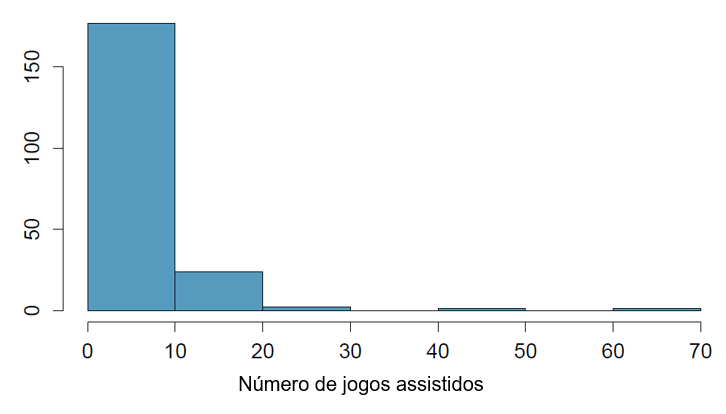
\includegraphics[width=0.8\textwidth]{4-4_clt/duke_games_pop.png}
\end{center}


\end{frame}


%%%%%%%%%%%%%%%%%%%%%%%%%%%%%%%%%%%

\begin{frame}[fragile]
\frametitle{Número médio de jogos de basquete (cont.)}
\justifying
Distribuição de amostras, n = 10:

\twocol{0.6}{0.4}{
\begin{center}
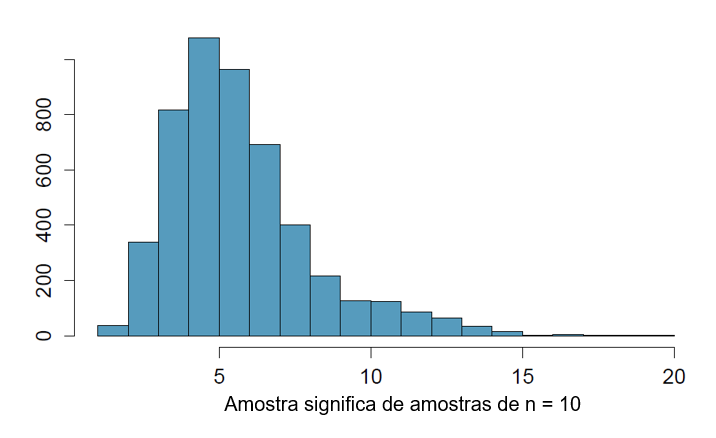
\includegraphics[width=\textwidth]{4-4_clt/duke_games_n10.png}
\end{center}
}
{\justifying
\dq{O que cada observação nesta distribuição representa??}
\justifying
\soln{\only<1>{\textcolor{white}{Média da amostra ($\bar{x}$) de amostras de tamanho $n = 10$.}}}
\justifying
\soln{\only<2->{Média da amostra ($\bar{x}$) de amostras de tamanho $n = 10$.}}

}

\end{frame}
%%%%%%%%%%%%%%%%%%%%%%%%%%%%%%%%%%%

\begin{frame}[fragile]
\frametitle{Número médio de jogos de basquete (cont.)}
\justifying
Distribuição de amostras, n = 10:

\twocol{0.6}{0.4}{
\begin{center}
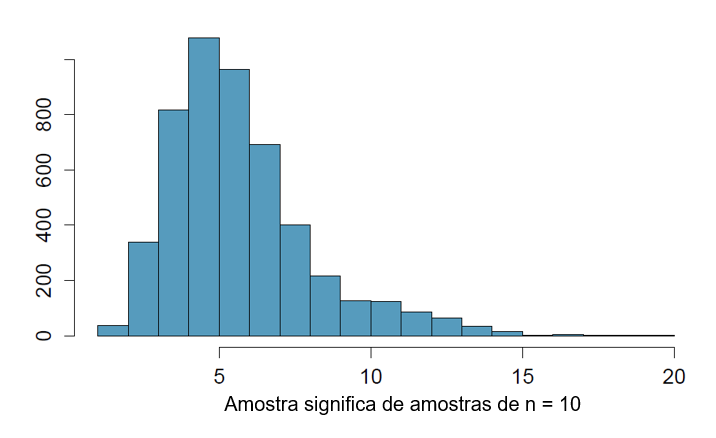
\includegraphics[width=\textwidth]{4-4_clt/duke_games_n10.png}
\end{center}
}
{\justifying
\dq{A variabilidade da distribuição amostral é menor ou maior que a variabilidade da distribuição populacional? Por quê?}
\justifying
\soln{\only<1-2>{\textcolor{white}{Menor, a média das amostras irá variar menos do que as observações individuais.}}}
\justifying
\soln{\only<3->{Menor, a média das amostras irá variar menos do que as observações individuais.}}
}

\end{frame}
%%%%%%%%%%%%%%%%%%%%%%%%%%%%%%%%%%%%

\begin{frame}[fragile]
\frametitle{Número médio de jogos de basquete (cont.)}
\justifying
Distribuição de amostras, n = 30:

\twocol{0.6}{0.4}{
\begin{center}
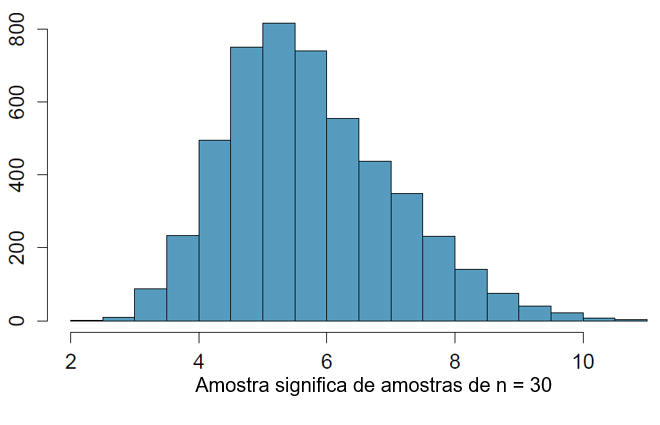
\includegraphics[width=\textwidth]{4-4_clt/duke_games_n30.png}
\end{center}
}
{\justifying
\dq{Como o formato, o centro e a disposição da distribuição amostral mudaram de $n = 10$ para $n = 30$?}
\justifying
\soln{\only<1>{\textcolor{white}{O formato é mais simétrico, o centro é aproximadamente o mesmo, a disposição é menor.}}}
\justifying
\soln{\only<2->{O formato é mais simétrico, o centro é aproximadamente o mesmo, a disposição é menor.}}
}

\end{frame}


%%%%%%%%%%%%%%%%%%%%%%%%%%%%%%%%%%%%

\begin{frame}[fragile]
\frametitle{Número médio de jogos de basquete (cont.)}
\justifying
Distribuição de amostras, n = 70:

\begin{center}
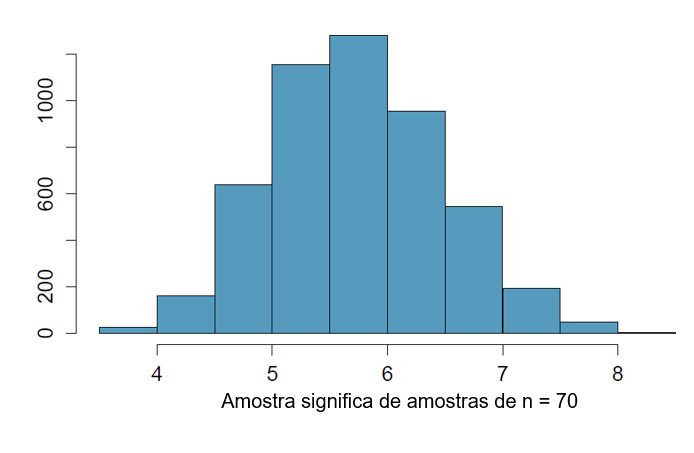
\includegraphics[width=0.6\textwidth]{4-4_clt/duke_games_n70.png}
\end{center}

\end{frame}


%%%%%%%%%%%%%%%%%%%%%%%%%%%%%%%%%%%%

\begin{frame}[fragile]
\frametitle{Número médio de jogos de basquete (cont.)}
\justifying
\dq{A média da distribuição amostral é de 5,75 e o desvio padrão da distribuição amostral (também chamado de \hl{erro padrão}) é 0,75. Qual dos seguintes opções é o palpite mais razoável para o intervalo de confiança de 95\% para o número médio real de jogos de basquete assistidos?}

\begin{enumerate}[(a)]
\item $5.75 \pm 0.75$
\solnMult{$5.75 \pm 2 \times 0.75$} \soln{\only<2>{\red{$\rightarrow (4.25,7.25)$}}}
\item $5.75 \pm 3 \times 0.75$
\item não podemos afirmar nada com as informações dadas.
\end{enumerate}


\end{frame}

%%%%%%%%%%%%%%%%%%%%%%%%%%%%%%%%%%%

\begin{frame}
\frametitle{Prática}
\justifying
\pq{
{ Quatro gráficos: determine qual gráficos (A, B ou C) é qual. \\
(1) No topo: distribuição para uma população ($\mu = 10, \sigma = 7$), \\
(2) uma única amostra aleatória de 100 observações dessa população, \\
(3) uma distribuição de 100 amostras de amostras aleatórias com tamanho 7, e \\
(4) uma distribuição de 100 amostras de amostras aleatórias com tamanho 49.}}

\end{frame}
%%%%%%%%%%%%%%%%%%%%%%%%%%%%%%%%%%%

\begin{frame}
\frametitle{Prática}

\twocol{0.4}{0.6}{
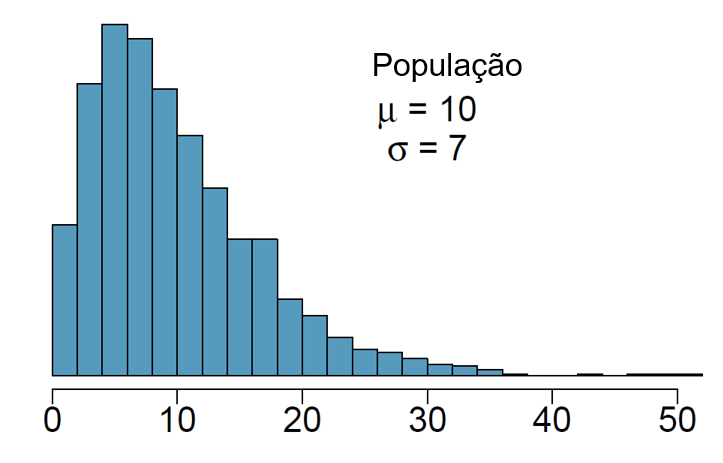
\includegraphics[width=\textwidth]{4-4_clt/cltSimRS_pop.png}
}
{
\vspace{-0.5cm}
{\small
\begin{enumerate}[(a)]
\solnMult{A - (3); B - (2); C - (4)}
\item A - (2); B - (3); C - (4)
\item A - (3); B - (4); C - (2)
\item A - (4); B - (2); C - (3)
\end{enumerate}
}
}
\vspace{-0.25cm}
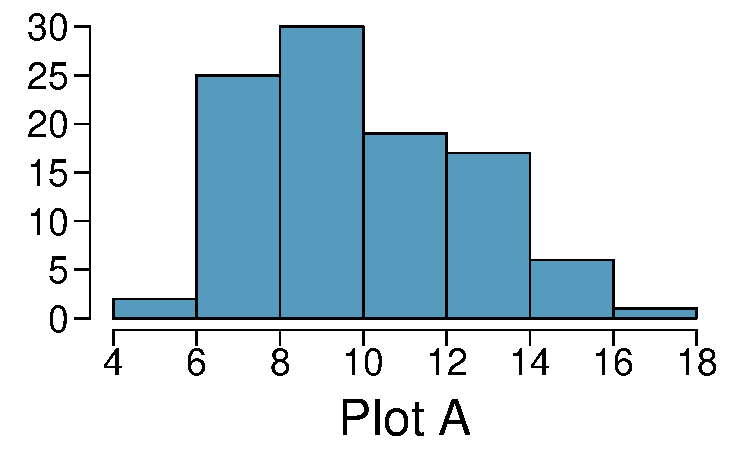
\includegraphics[width=0.32\textwidth]{4-4_clt/cltSimRS_n7.pdf}
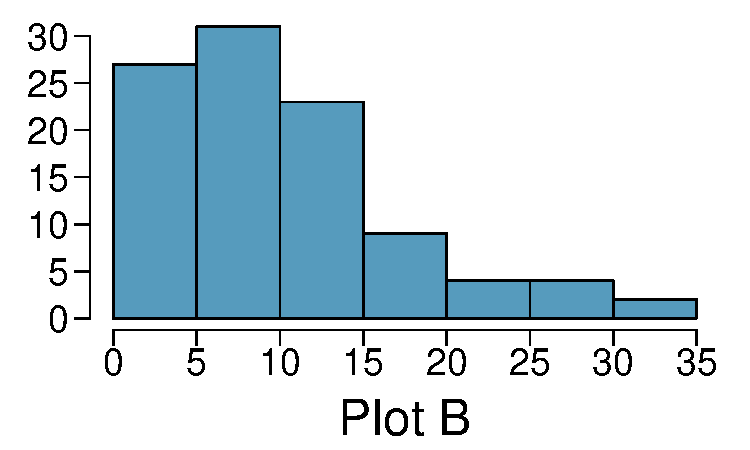
\includegraphics[width=0.32\textwidth]{4-4_clt/cltSimRS_samp.pdf}
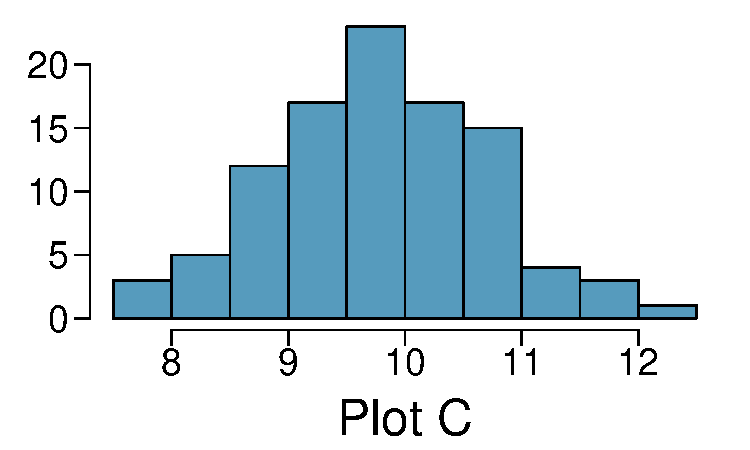
\includegraphics[width=0.32\textwidth]{4-4_clt/cltSimRS_n49.pdf}

\end{frame}

%%%%%%%%%%%%%%%%%%%%%%%%%%%%%%%%%%%%

